\documentclass[12pt, a4paper]{article}
\usepackage[utf8]{inputenc}
\usepackage{graphicx}
\usepackage{gensymb}
\usepackage{amsmath}
\usepackage{float}
\usepackage[figurename=Graf]{caption}
\usepackage{subcaption}
\usepackage{caption}


\title{Lastne vrednosti in lastni vektorji}
\author{Miha Pompe}
\date{Oktober 2021}

\begin{document}
\begin{titlepage}
	\centering
 	
\includegraphics[width=0.45\textwidth]{logo_fmf_uni-lj_sl_veliki.png}\par\vspace{1cm}

	\vspace{1cm}

	\vspace{1.5cm}
	{\huge\bfseries Lastne vrednosti in lastni vektorji\par}
	\vspace{2cm}
	{\Large Miha Pompe 28191072\par}
	\vfill

	\vfill

% Bottom of the page
	{\large Oktober 2021\par}
\end{titlepage}
% \maketitle
\thispagestyle{empty}
\clearpage
\pagenumbering{arabic}
\newpage


\section{Uvod}
Enodimenzionalni linearni harmonski oscilator (delec mase $m$
s kinetično energijo $T(p)=p^2/2m$ v kvadratičnem potencialu
$V(q)=m\omega^2 q^2/2$) opišemo z brezdimenzijsko Hamiltonovo funkcijo
\begin{equation*}
  H_0 = {1\over 2} \left( p^2 + q^2 \right) \>,
\end{equation*}
tako da energijo merimo v enotah $\hbar\omega$, gibalne količine
v enotah $(\hbar m\omega)^{1/2}$ in dolžine v enotah $(\hbar/m\omega)^{1/2}$.
Lastna stanja $|n\rangle$ nemotenega Hamiltonovega operatorja $H_0$ so
\begin{equation*}
  |n\rangle = (2^n n! \sqrt{\pi})^{-1/2} \mathrm{e}^{-q^2/2}\,  {\cal H}_n (q)\>,
\end{equation*}
kjer so ${\cal H}_n$ Hermitovi polinomi.
Lastne funkcije zadoščajo stacionarni Schr\"odingerjevi enačbi
\begin{equation*}
H_0 | n^0 \rangle = E_n^0 | n^0 \rangle
\end{equation*}
z nedegeneriranimi lastnimi energijami $E_n^0 = n + 1/2$
za $n=0,1,2,\ldots~$.  Matrika $\langle i | H_0 | j\rangle$
z $i,j=0,1,2,\ldots,N-1$ je diagonalna, z vrednostmi
$\delta_{ij}(i + 1/2)$ po diagonali.  Nemoteni Hamiltonki
dodamo anharmonski člen
\begin{equation*}
H = H_0 + \lambda q^4 \>.
\end{equation*}
Matriko s tem potencialom v nadaljevanju navajamo s $H$. Tedaj matriko zapišemo kot
\begin{equation*}
  \langle  i | H | j \rangle = \langle  i | H_0 | j \rangle + \lambda \langle  i | q^4 | j \rangle
\end{equation*}
Za izračun drugega člena si lahko pomagamo z naslednjimi zvezami
\begin{align*}
  &\langle i | q | j \rangle = {1\over 2} \sqrt{i+j+1}\,\, \delta_{|i-j|,1} \\
  &\langle i|q^2|j\rangle
  = {1\over 2} \biggl[
    {\sqrt{j(j-1)}} \, \delta_{i,j-2}
  + {(2j+1)} \, \delta_{i,j}
  + {\sqrt{(j+1)(j+2)}} \, \delta_{i,j+2} \biggr] \\
  &\langle i|q^4|j\rangle
  = {1\over 2^4}\sqrt{2^i \, i!\over 2^{j} \, j! } \, \biggl[ \,
  \delta_{i,j+4} + 4\left(2j+3\right) \delta_{i,j+2}
                      + 12 \left(2j^2+2j+1\right) \, \delta_{i,j} \\[3pt]
  &+ 16j \left(2j^2-3j+1\right) \, \delta_{i,j-2}
     + 16j\left(j^3-6j^2+11j-6\right) \, \delta_{i,j-4} \biggr]
\end{align*}
Sedaj rešujemo matrični sistem
\begin{equation*}
  H | n \rangle = E_n | n \rangle \>.
\end{equation*}
katerega bomo reševali v basi lastnih funkcij harmonskega oscilatorja $| i \rangle$:
\begin{equation*}
  | n \rangle = \sum_{i=0}^N c_i | i \rangle
\end{equation*}
Metodo lahko nato prenesemo na drugačne potenciale. V tem delu je analiziran še naslednji
\begin{equation*}
  H = {p^2\over 2} - 2q^2 + {q^4\over 10} \>.
\end{equation*}
Podobno kot prej lahko matriko zapišemo kot
\begin{equation*}
  \langle  i | H | j \rangle = \langle  i | H_0 | j \rangle - \frac{5}{2} \langle  i | q^2 | j \rangle + \frac{1}{10} \langle  i | q^4 | j \rangle
\end{equation*}
Matriko s tem potencialom v nadaljevanju navajamo s $H_2$.


\section{Postopek}
Implementacija postopka se deli na dva dela; generiranje matrike $H$ in diagonalizacija. Matrične elemente lahko hitro generiramo z uporabo paketa {\sc numpy}, ki nam omogoča hiter izračun funkcije na celotnem vektorju. Ta vektor predstavlja koordinate matrike, funkcije za izračun elementov pa so podane v Uvodu. Problem se pojavi pri računanju $\langle  i | q^4 | j \rangle$ saj v formuli nastopa količnik fakultet. Preprosta implementacija hitro divergira pri velikih matrikah, zato lahko količnik implementiramo kot samostojno funkcijo, pri čemer pa ne moremo uporabljati prednosti numeričnega paketa {\sc numpy}. Graf 1a prikazuje čas izračuna v odvisnosti od velikost in izbire metode, pri čemer lahko opazimo razliko v časovni zahtevnosti. Primerjamo lahko tudi napako drugih implementacij in sicer dobimo, da je povprečje relativnih napak metode $[q_{ij}^2]^2$ enako $0.37\%$ in metode $[q_{ij}]^4$ je enako $1.31\%$, merjeno za matriko velikosti $N=100$. Graf 1b predstavlja vrednosti Hamiltonove matrike pri uporabi različnih metod.\\
\begin{figure}[hbtp]
  \centering
  \begin{subfigure}{\textwidth}
    \centering 
    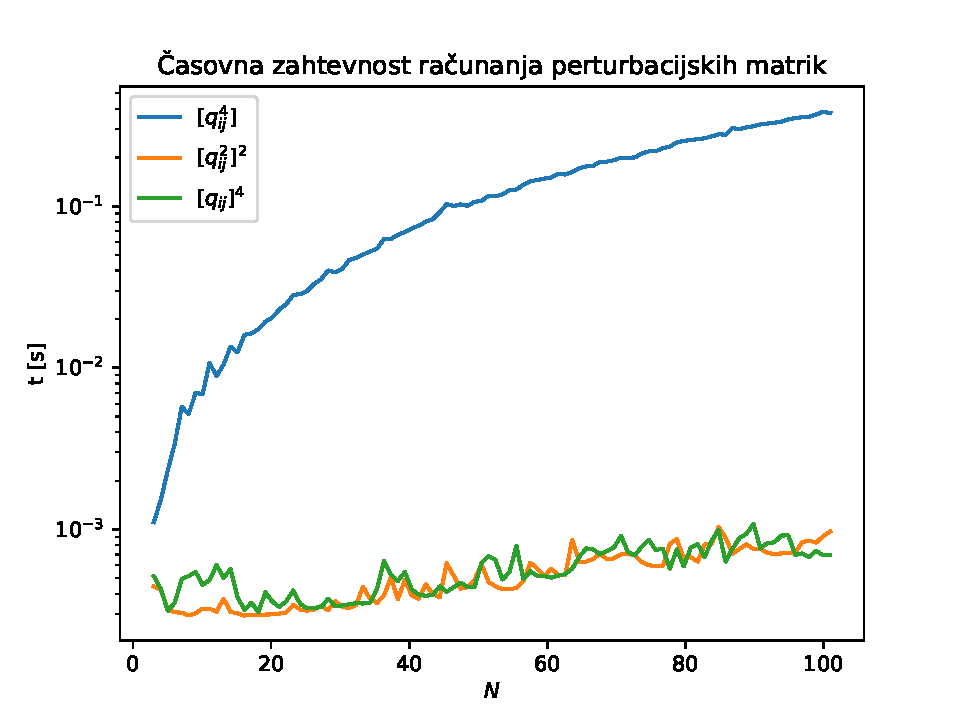
\includegraphics[width=\linewidth]{grafi/q_vs_N.pdf}
    \caption{Čas generiranja matrike $\langle  i | q^4 | j \rangle$ v odvisnosti od velikosti in izbire metode.}
    \label{fig:sub1}
  \end{subfigure} 
  \begin{subfigure}{\textwidth}
    \centering
    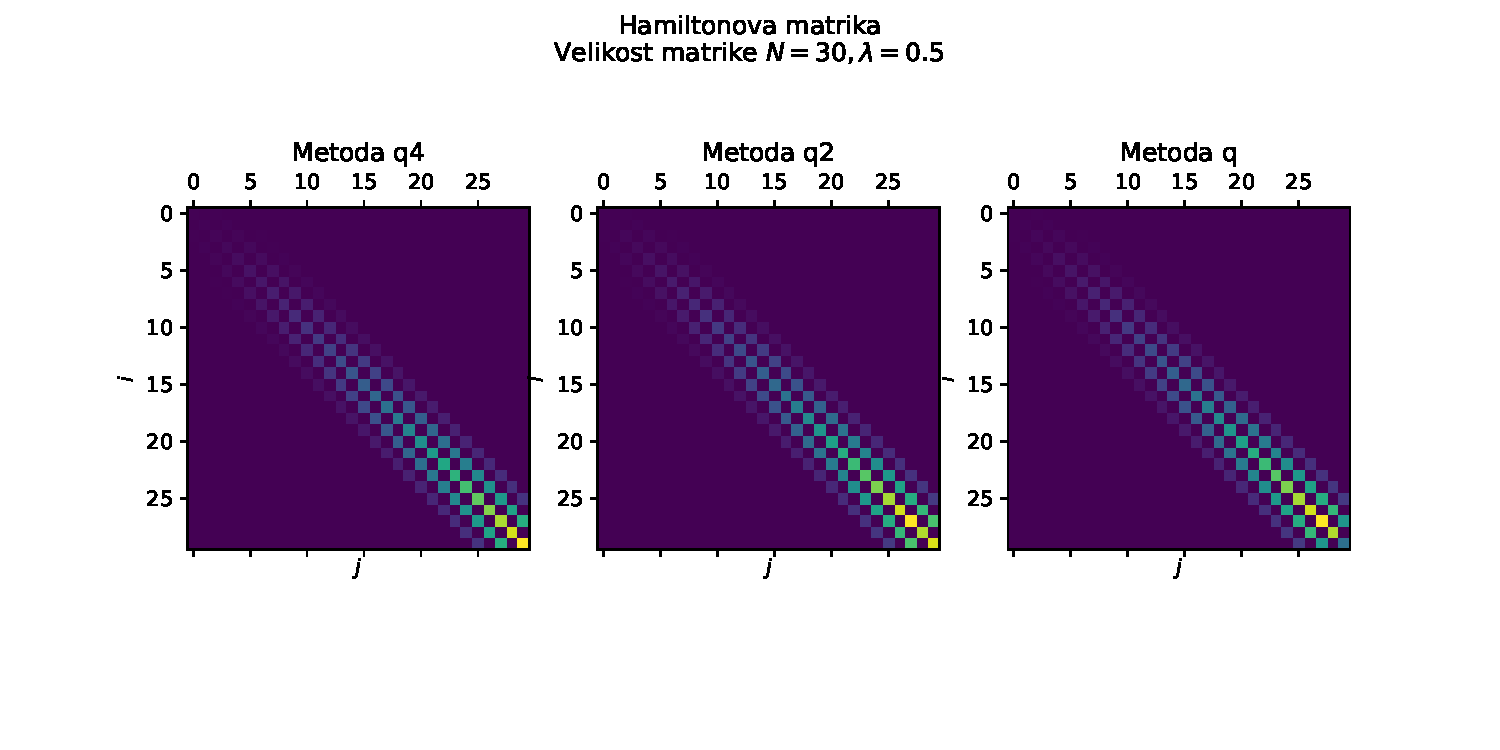
\includegraphics[width=\linewidth]{grafi/matrika.pdf}
    \caption{Vizualizacija matrike $H$ z uporabo naslednjih metod za izračun $\langle  i | q^4 | j \rangle$: $[q_{ij}^4]$, $[q_{ij}^2]^2$ in $[q_{ij}]^4$.}
    \label{fig:sub2}
  \end{subfigure}   
  \caption{Lastnosti implementacije generiranja matrike $H$.}
  \label{fig:test}
\end{figure}

Drugi del postopka je diagonalizacija matrike $H$, pri čemer izračunamo lastne vrednosti in lastne vektorje matrike. Diagonalizacijo smo izvedli s tremi različnimi metodami:
\begin{itemize}
  \item Householderjeva metoda tridiagonalizacije s sledečo QR iteracijo (Householderjeva zrcaljenja), 
  v nadaljevanju imenovana Householder
  \item Householderjeva metoda tridiagonalizacije s sledečo QR iteracija ({\sc numpy.\-linalg.qr}), 
  v nadaljevanju imenovana Numpy QR oz. Numpy tri diag,
  \item diagonalizacija z uporabo vgrajene funkcije {\sc numpy.linalg.eig}, 
  v nadaljevanju imenovana Numpy diag.
\end{itemize} 
Analiza izbranih metod je navedena v poglavju Rezultati.

\section{Rezultati}
  
Glavni del naloge je primerjava metod diagonalizacije in analiza vrednosti. Kot referenčna metoda je bila izbrana funkcije {\sc numpy.linalg.eig}, veljavnost katere je bila preverjena na manjših in preprostih matrikah. Rezultate sem primerjal diagonalizacijo matematičnega programa Mathematica. Grafa 2c in 2d prikazujeta relativno napako največje lastne vrednosti. Opazimo, da je najnižja napaka pri manjših matrikah in se nato povečuje z velikostjo, od določene točke naprej napaka ponovno pada. Vidimo tudi, da se napaki obeh implementacij zelo skladata, iz česar lahko sklepamo, da napaka izvira iz postopka tridiagonalizacije, ki je skupna obema metodama.\\

Časovna zahtevnost diagonalizacije raste z velikostjo matrike. Zaradi učinkovitosti paketa {\sc numpy} sta zadnji dve metodi bolj učinkoviti kot Householderjeva. Metoda Numpy QR pa je počasnejša od Numpy diag saj algoritem vsebuje Householderjevo tridiagonalizacijo. Ročno napisane metode so počasnejše zaradi uporabe počasnih for zank.\\

Lastne vrednosti so sorazmerne z energijami lastnih stanj, iz Grafa 2a pa lahko opazimo da so te vrednosti odvisne tudi od velikosti matrike $H$. Tu abscisna os predstavlja n-to lastno vrednost, ordinata pa velikost n-te lasten vrednosti. Lastne vrednosti ne naraščajo linearno kot pri harmonskem oscilatorju temveč potenčno. Za vsako lastno vrednost pa lahko izračunamo tudi lastni vektor, katerega na Grafu 3 predstavimo v funkcijski obliki.\\

Primerjajmo še lastne vrednosti različnih potencialov. Kot že vemo lastne vrednosti harmonskega oscilatorja ($H_0$) naraščajo linearno in anharmonskega ($H$) potenčno, poglejmo še potencial z dvema minimumoma ($H_2$). Le-tu ponovno opazimo potenčno naraščanje, vendar počasneje kot pri $H$. Nižje lastne vrednosti so negativne, saj je tudi del potenciala negativen.\\

  
\begin{figure}[hbtp]
  \begin{center}
  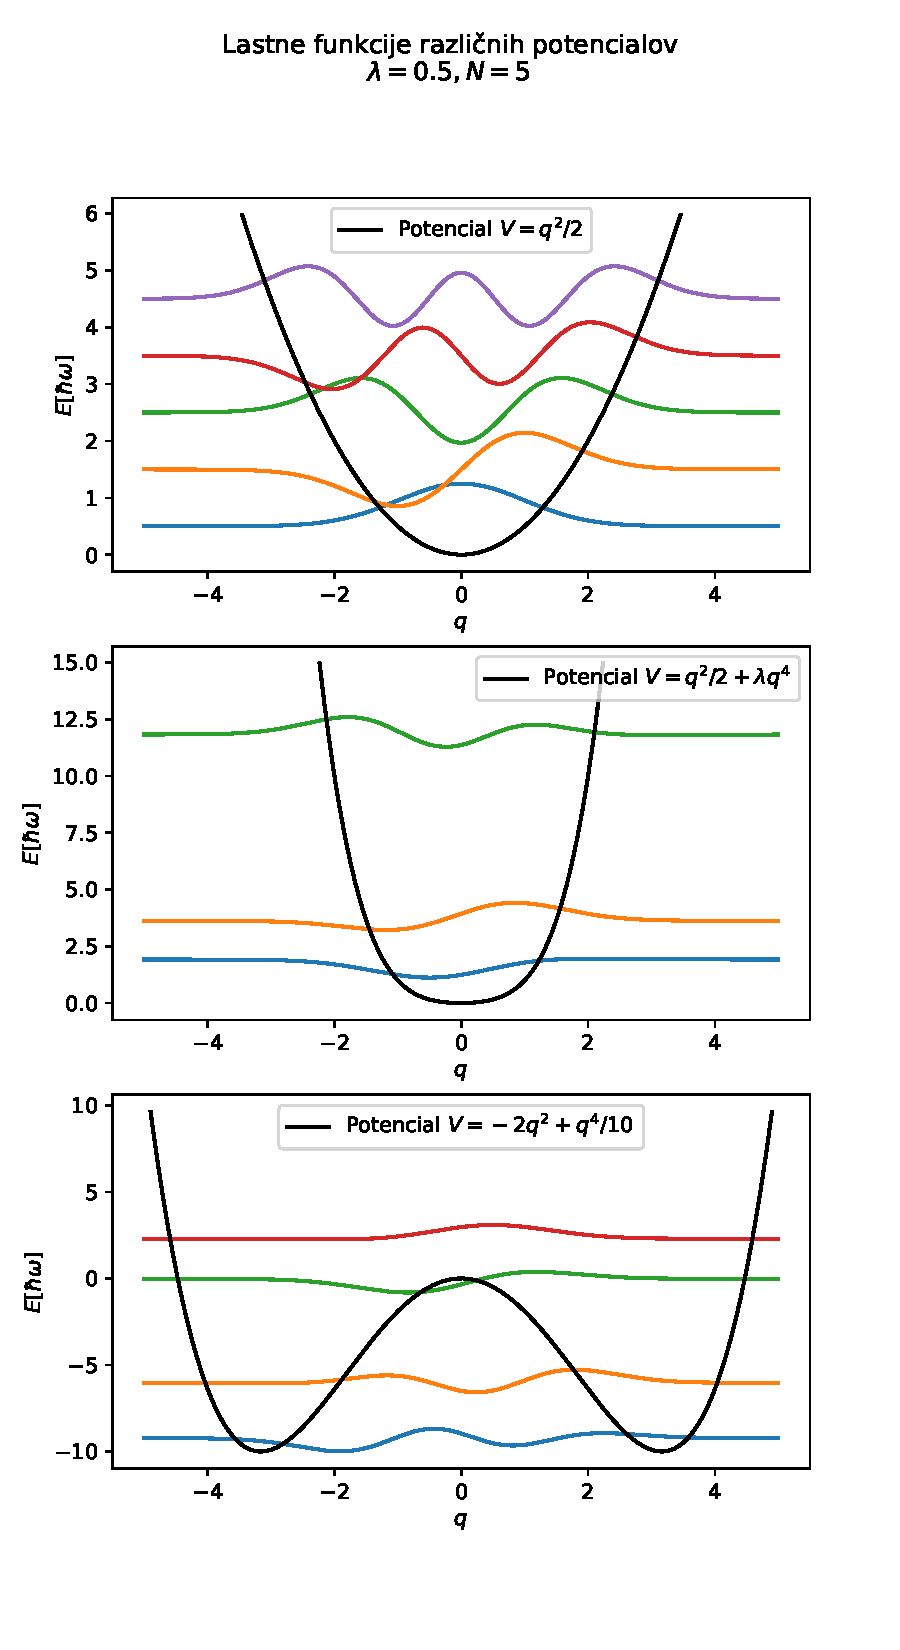
\includegraphics[width=0.8\linewidth]{grafi/lastne_f_vs_potenciali.pdf}
  \caption{Lastne funkcije različnih potencialov.}
  \end{center}
\end{figure}

\end{document}

